%!TEX root = practicum2.tex
Given a dichotomy $\mathcal{D} = \left\{\xi^i, S^i \right\}_{i}^{P}$ with $P$ $N$-dimensional patterns $\xi \in \mathcal{R}^N$. The labels $S$ were assigned by a teacher perceptron according to:

\begin{equation}\label{eq:method:teacher_label}
	S^\mu = \text{sign}(\vec{w}^* \cdot {\vec{\xi}}^{\mu})
\end{equation}

The teacher $\vec{w}^*$ can be chosen randomly as long as the following condition holds:
\begin{equation}\label{eq:method:teachervectorcondition}
	\norm{\vec{w}^*}^2 = N.
\end{equation}

\begin{figure}
	\centering
	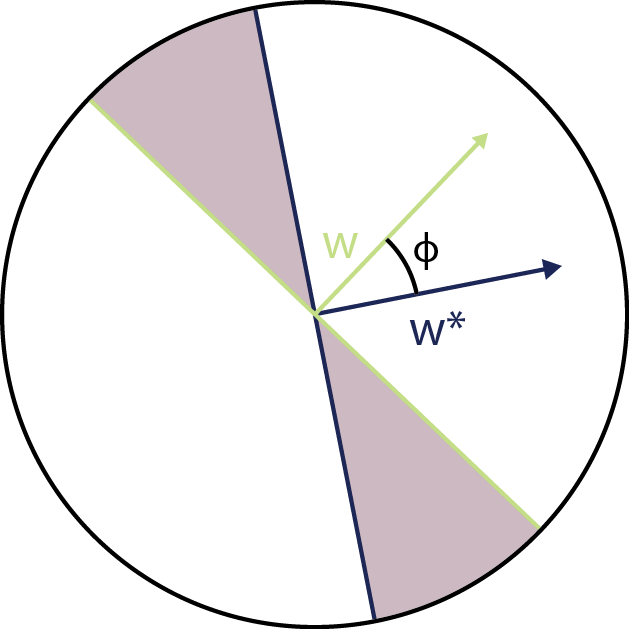
\includegraphics[scale=1]{./img/generalizationError}
	\caption{The difference between two vectors $\vec{w_1}$ and $\vec{w_2}$.} 
	\label{fig:methode:generalizationError}
\end{figure}

~\\To compare two weight vectors $\vec{w_1}$ and $\vec{w_2}$ we use the probability that $\vec{w_1}$ classifies a pattern $\vec{\xi}$ different then $\vec{w_2}$. The shaded area in \cref{fig:methode:generalizationError} shows the probability that $\vec{w_1}$ and $\vec{w_2}$ disagree. Denoting the angle between the two vectors with $\phi$, the probability of the two vectors disagreeing can be written as:
	\begin{equation}\label{eq:method:generalizationError1}
		\epsilon = \frac{2\phi}{2\pi}.
	\end{equation}
\clearpage
\noindent Using the following definition of the dot product:
	\begin{equation}\label{eq::method:dotProduct}
		\vec{a} \cdot \vec{b} = \norm{a} \norm{b} \cos \phi,
	\end{equation}
we rewrite \eqref{eq:method:generalizationError1} to:
	\begin{equation}\label{eq:method:generalizationError2}
		\epsilon = \frac{1}{\pi} \arccos \left(\frac{\vec{w} \cdot \vec{w}^*}{\norm{\vec{w}} \norm{\vec{w}^*}}\right).
	\end{equation}

~\\The Minover algorithm is an iterative procedure that tries to find the weight vector of maximal stability. The stability of a pattern $\vec{\xi^\mu}$ given weight vector $\vec{w}$ is defined as: 

\begin{equation}\label{eq:method:maximum_stability}
	\kappa^\mu = \frac{\vec{w} \cdot \vec{\xi} \cdot S}{\norm{\vec{w}}}.
\end{equation}

The stability defined in \eqref{eq:method:maximum_stability} can be thought of as the distance between a pattern and the current weight vector $\vec{w}(t)$. 

To eventually find the weight vector with maximal stability the algorithm takes the following two steps every iteration: it selects the pattern $\mu(t)$ with the minimal distance/stability (minimal overlap) to the current solution. The current weight vector $\vec{w}(t)$ is then updated with Hebb's rule, see \eqref{eq:method:update}. 

	\begin{equation}\label{eq:method:update}
		\vec{w}(t + 1) = \vec{w}(t) + \frac{1}{N} \xi^{\mu(t)} S^{\mu(t)} 
	\end{equation}

The stability of a perceptron for a given dichotomy $\mathcal{D}$ is:
	\begin{equation}
		\kappa(\vec{w}) = \min_{\mu} \left\{ \kappa^\mu \right\}.
	\end{equation}

~\\The Minover algorithm terminates when either the weight vector does not change anymore for $P$ steps or the number of maximal time steps $t_{max} = n_{max} \cdot P$ has been reached. Where $n_{max}$ is comparable to the number of epochs in the Rosenblatt algorithm. 

To compare the weight vectors $\vec{w}(t)$ and $\vec{w}(t - 1)$ we use the error measure defined in \eqref{eq:method:generalizationError2}. We say that a weight vector has not changed for $P$ steps if $\epsilon$ for the last $P$ weight vectors differentiates less than $0 \pm \varepsilon$.

See \autoref{alg:method:minnover} for the pseudo code of the procedure described above. The method \texttt{notConverged} compares the differences between the last $P$ weight vectors using \eqref{eq:method:generalizationError2} as explained earlier.

%!TEX root = practicum3.tex		
\begin{algorithm}
	\setstretch{1.2}
	\SetAlgoShortEnd
	\DontPrintSemicolon
	\SetKwInOut{Input}{input}\SetKwInOut{Output}{output}
	\Input{
		${\mathcal{D} = \left\{ \vec{\xi}^\mu, \tau\left(\vec{\xi}^\mu\right) \right\}_{\mu = 1}^{P}}$\\
		$t_{max}$ maximum number of epochs\\
		$\eta$ the learning rate
	}
	\Output{$\vec{w}^1$, $\vec{w}^2$ the weights}
	\BlankLine

	$[\vec{w}^1, \vec{w}^2]$ := \FuncSty{init($D$)} \tcc*{$\norm{\vec{w}}^2 = 1$}

	\For{$t \leftarrow 1$ \KwTo $t_{max}$}{
		\For{$i \leftarrow 1$ \KwTo $P$}{
			$\mu$ := \FuncSty{get\_random\_pattern()}\;
			$[\vec{w}^1, \vec{w}^2]$ := \FuncSty{update($\mu$)} \tcc*{\eqref{eq:1:update}}
		}
	}
	\caption{$SGD(\mathcal{D}, t_{max}, \eta)$\label{alg:method}}
\end{algorithm}

An implementation of the pseudo code in \autoref{alg:method:minnover} can be found in \cref{ap:matlab}.

As stated before Minover, contrary to Rosenblatt, does not stop when a solution is found but continues until the solution with optimal stability is found. The advantage of this is that the perceptron trained using the Minimal Overlap algorithm generalizes better. 

